\documentclass[letterpaper,oneside]{scrartcl}
\usepackage{fullpage}
\usepackage[utf8]{inputenc}
\usepackage[pdftex]{graphicx}
\DeclareGraphicsExtensions{.png,.pdf}
\graphicspath{{plots/}}
\usepackage{hyperref}
\usepackage{url}
\usepackage[round,sectionbib]{natbib}
\bibliographystyle{abbrvnat}
\usepackage[small]{caption2}
\usepackage[small]{titlesec}
\renewcommand\familydefault{bch}

\title{Product graphics}
\author{Heike Hofmann and Hadley Wickham}
\begin{document}
\maketitle
  
\section{Introduction}


The Grammar of Graphics [reference] is a grammar describing the components of statistical graphics and how they can be combined together.  These components are very flexible and can be used to describe any type of plot.  However, the book (Grammar with a capital G) does not present many examples of graphics for categorical data, and in those examples the use of the grammar gives little insight into plot.  This paper describes common categorical plots, and presents a specialisation of the Grammar of Graphics specifically designed to describe these types of plots and give insight into the types of relationships that they can show.  

Area plots [reference] display categorical data with a rectangle for each combination of the factors of interest, with the area of the rectangle proportional to the number of observations in that combination.  The layout of the rectangles give rise to the difference categorical plots that we are familiar with: bar charts, spine charts, mosaic plots, equal-bin-size plots, and fluctuation diagrams.  Trellis graphics are another type of display that uses categorical variables to create small multiples for different subsets of the data.  Visually, trellis graphics look like equal-bin-size plots with another plot drawn inside each bin.  Figure \ref{fig:cat-examples} illustrates some of these plots.

\begin{figure}[htbp]
  \begin{center}
  %  \includegraphics[scale=1]{file}
  \end{center}
  \caption{Area plot examples.}
  \label{fig:cat-examples}
\end{figure}

Area plots are the graphical equivalent to contingency tables.  And like contingency tables, they can be used to display raw counts, or to display proportions or percentages.  Similarly, it may be useful to augment area plots with marginal displays as we augment contingency tables with marginal sums.

Area plots different to other types of graphics, because must be able to flexible change level of aggregation.  Values are typically counts, but can also be sums of observation level weights.

These techniques can also be used with continuous data, if the data is binned to create a categorical variable.  This gives rise to the histogram and spinogram, analogues of the bar chart and spine chart respectively.  A long standing tradition is that no gaps are displayed between adjacent rectangles when used for originally continuous data.  Two examples are shown in Figure \ref{fig:cont-examples}.

\begin{figure}[htbp]
  \begin{center}
  \end{center}
  \caption{Area plots of originally continuous data}
  \label{fig:cont-examples}
\end{figure}

These techniques are also closely related to TreeMaps and dimensional stacking \citep{leblanc:1990}

What are the common components of all these plots, and how can be describe them in a succinct way that also allows us to describe what tasks each display is good for?  We propose that there is one key feature that makes these plots special.  That is there their coordinate system, which is hierarchical.  

In most coordinate systems that we are used to, such as Cartesian or polar coordinates, are symmetric in the sense that you can locate a point by starting from either dimension.  For example, in Cartesian coordinates you can identify either the x- or y-coordinate first, and the other next.  This also implies a distance symmetry when projected onto 2D Euclidean geometry. When you vary one coordinate by a small amount (holding all others constant) points in the projective geometry will be close.

Neither of these properties hold for hierarchical coordinate systems. 

We will discuss hierachical coordinate systems in general, and then present a specific hierachical coordinate system which gives rise to the area plots described previously.  We also present an R implementation, in the R package {\tt ggplot}.

Related work:

\citep{vliegen:2006}
\citep{ahlberg:1996}


\citep{hartigan:1984,hartigan:1981}
\citep{friendly:1999,friendly:1994}
\citep{theus:1999}
\citep{hofmann:2000,hofmann:2001,hofmann:2003}

Goals:

\begin{itemize}
  \item Put all area plots (bar charts, spine plots, mosaic plots, fluctuation diagrams) on a common footing
  \item Continue to build link between graphics and log-linear models
  \item Provide tools for ``residuals and re-iteration''
\end{itemize}  

Basic idea is factorising table of probabilities:

\begin{itemize}
  \item as products of marginal and conditional distributions
  \item as areas in plots
  \item as sums of parameters in log-linear models
\end{itemize}


\section{Data}
\label{sec:data}

To illustrate the techniques in this paper, we'll use a small sample from the general social survey ({\sc gss}) focussing on happiness.  51\,020 observations from a yearly survey from 1972 to 2006.  Happy, age, sex, marital status, terminal education level, relative financial status and health.  Also contains a weighting variable wtssall, which is a probability weight from the survey.

\subsection{Factorising probabilities}

Let $f(x, y, z)$ be the 2d pmf function generated.  Can write this pmf as product of marginals and conditionals

\begin{itemize}
  \item $f(x, y, z) = f(x, y | z) f(z)$
  \item $f(x, y, z) = f(x | y, z) f(y, z)$
  \item $f(x, y, z) = f(x | y, z) f(y | z) f(z)$
\end{itemize}

Compare to area of mosaic plot.

One other special 2d case is the equal bin size plot - which all 1d x 1d primitive plots collapse down to when counts are equal.  The important difference is the formatting - a grid rather than nested boxes.

\subsection{Weighting}
\label{sub:weighting}

We have assumed the probabilities represent counts, but WLOG we can use any set of non-negative additive weights instead.  Some of the applications of such weighted plots are described in \citet{unwin:2007}.

\subsection{Continuous data}
\label{sub:continuous_data}

Binning. 

Convention when using binned continuous data is to remove the gap between regions.

\subsection{Nested data}
\label{sub:nested_data}

\section{Display}
\label{sec:display}


The three plots above are special cases of $a(i, j) = w(i, j)^x * h(i, j)^y$.  $x + y = 1$.

Perceptual constraints.  Best at comparing area when:

\begin{itemize}
  \item Simple shape (i.e. square vs polygon)
  \item Aspect ratios similar
  \item Areas are large
  \item Areas are close
  \item One border is constant.
\end{itemize}

Impossible to simultaneously satisfy all constraints.  Every product plot requires the creator to trade off between these.

Restrictions on partitioning

\begin{itemize}
  \item Area should be proportional to weight
  \item Containment
  \item Rectangular
  \item Non-overlapping
\end{itemize}

Pseudo 2d, where you take a long 1d structure and wrap it into 2d.

Pseduo 1d, where you make a new variable from multiple variables.

\subsection{1d primitives}

Space-filling vs. not space-filling.  Read length on common scale, vs. put more information in the display.

Basic principle of all area plots is area should be proportional to probability. For the plots we are interested in, the shape used to represent the count is a rectangle, so that $a(i, j) = w(i, j) * h(i, j)$. Each plot type constrains this relationship in a different way:

\begin{itemize}
  \item {\bf bar}: height is proportional to value, width equally divides space. Bars allow comparison between absolute numbers.

  \item {\bf spine}: width is proportional to value, height equally divides space. Spines not useful at top level, but allow comparison of proportions at next level (ie. conditioned on top level values)

  \item {\bf treemap}: no restrictions on height and width.

\end{itemize}

\subsection{2d primitives}

\begin{itemize}
  \item {\bf fluct}: width and height proportional to square root of value. Flucts allow comparisons of (approximately) absolute numbers in two directions. 
  
\end{itemize}

\subsection{Plot templates}

\begin{itemize}
  \item {\bf Stacked} barchart: 1 bar + $n-1$ spines in opposite direction.
  \item {\bf Nested} barchart: $n$ bars.
  \item {\bf Mosaic} plot: spines in alternating directions.  The 1d case has a special name, the spineplot.
  \item {\bf Double-decker} plot: $n-1$ spines + 1 spine in opposite direction.
  
  \item {\bf Fluctuation} diagram: 
\end{itemize}



\subsection{Violation of constraints}

\subsubsection{Small values and zeros}
\subsubsection{Cascading}

The cascaded treemaps of \citet{lu:2008} is an idea that illustrates how the violation of containment can be productive.  In the cascaded treemap, each level is slightly offset from the one above to create a pseudo-3d perspective.

\subsubsection{Non-rectangular partitions}

Pie charts fall out naturally, as bars in polar coordinates, with angle and radius instead of height and width. And to ensure that counts stay proportional to areas, the square-root is taken of the y-axis. This is related to the infoslices of \citet{andrews:1998}, which only use half of the disk. Figure~\ref{fig:polar} shows some examples of product plots in polar coordinates.

\begin{itemize}
  \item Pie charts
  \item Fourfold displays \citep{friendly:1995}
  \item Bullseye chart
\end{itemize}

\begin{figure}[htbp]
  \centering
    \includegraphics[width=0.25\linewidth]{hb-vb-cartesian}%
    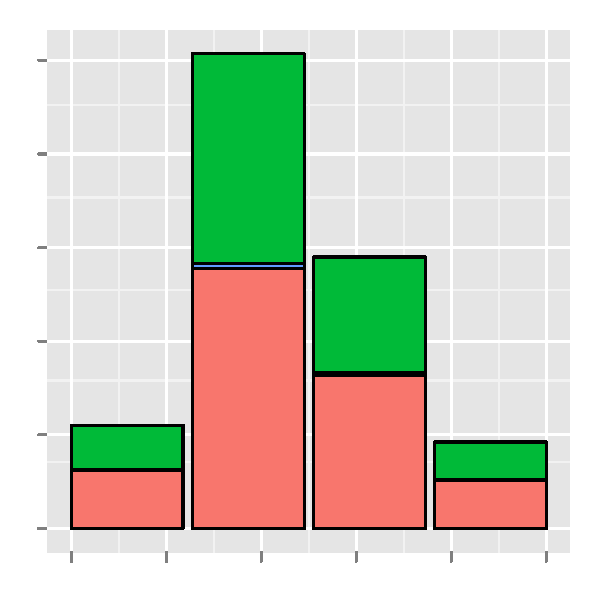
\includegraphics[width=0.25\linewidth]{hb-vs-cartesian}%
    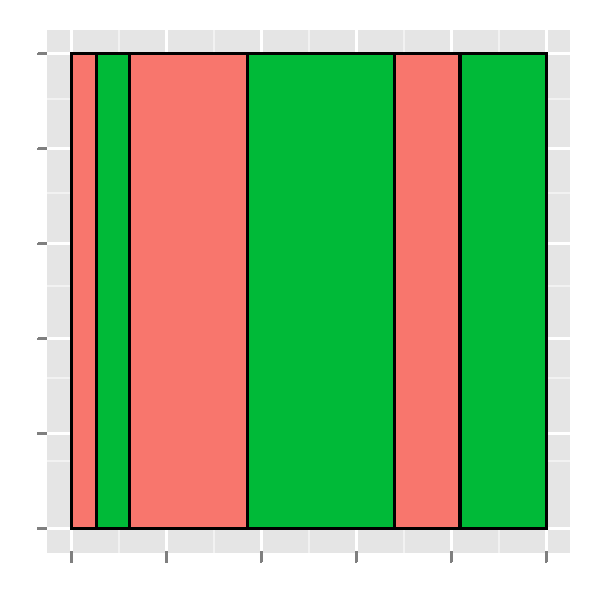
\includegraphics[width=0.25\linewidth]{hs-hs-cartesian}%
    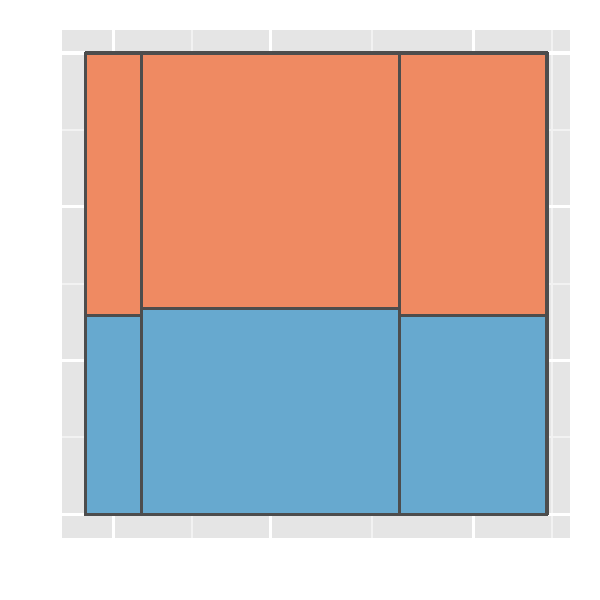
\includegraphics[width=0.25\linewidth]{hs-vs-cartesian}

    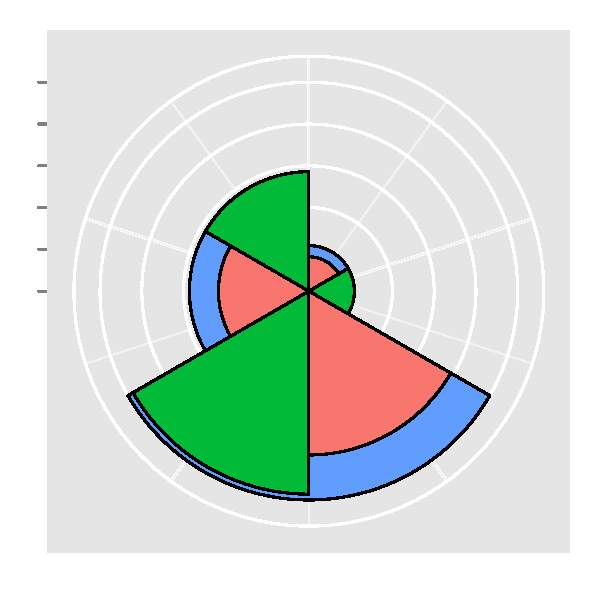
\includegraphics[width=0.25\linewidth]{hb-vb-polar}%
    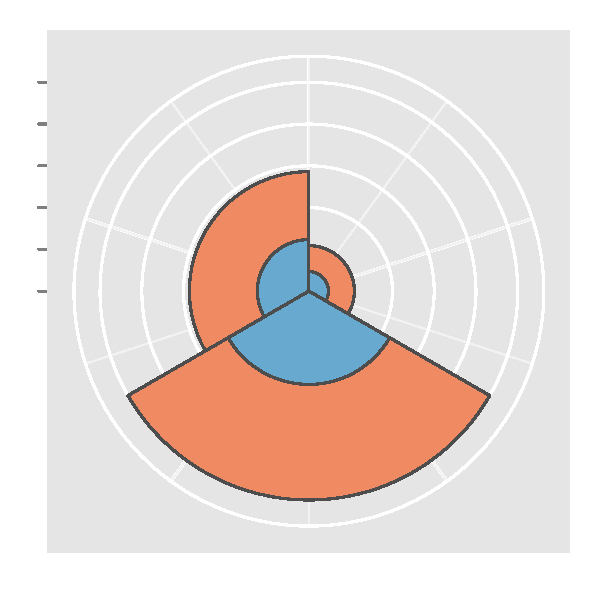
\includegraphics[width=0.25\linewidth]{hb-vs-polar}%
    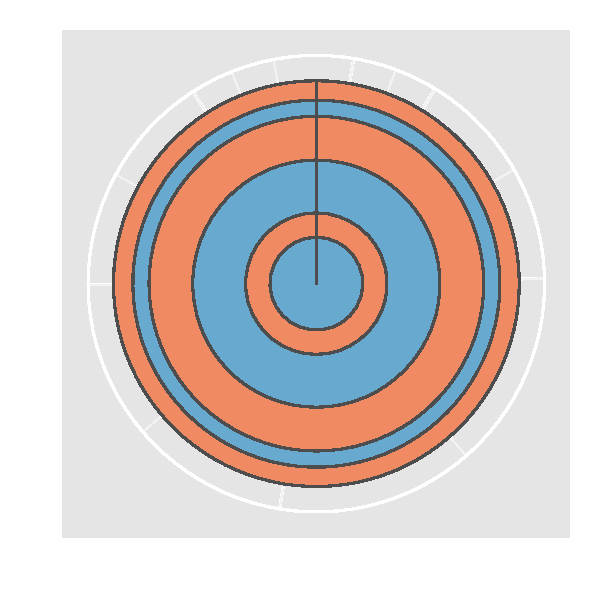
\includegraphics[width=0.25\linewidth]{hs-hs-polar}%
    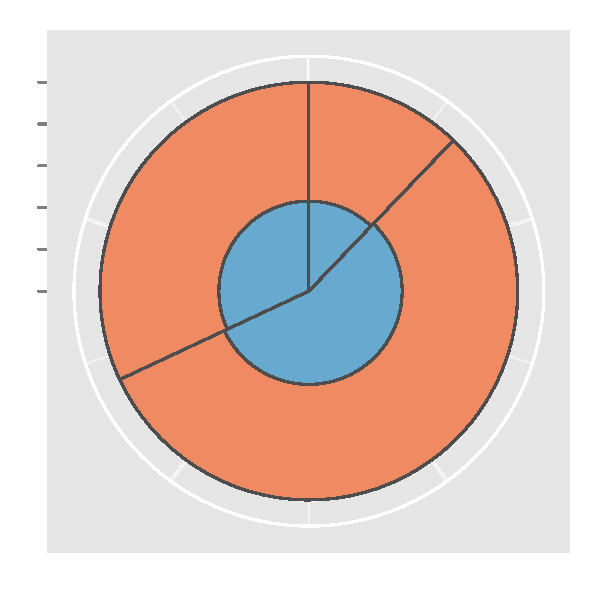
\includegraphics[width=0.25\linewidth]{hs-vs-polar}
  \caption{}
  \label{fig:polar}
\end{figure}

Circular treemaps of \citet{wetzel:2008} which use circles instead of rectangles, but is not space filling because you can not tile a circular region with circles. The radial displays of \citet{stasko:2000} deliberately keep the radius constant in order to relatively highlight the lower levels.  Similarly so does the fanlens of \citet{lou:2007}

Other non-rectangular treemaps have been proposed, such as the space-filling curve approach of \citep{wattenberg:2005}, or the voronoi treemaps of \citep{wattenberg:2005}, but because of the perceptual difficultly of comparing areas of arbitrary polygons, these approaches tend to be attractive rather than useful.


\section{Connection with log-linear models}
\label{sec:models}



which imply the obvious mapping between d(i, j) and a(i, j).  For >2d,
the definitions generalise in the obvious, but the constraints become
more complicated.

$log(d(i,j)) = 1 + d_{i \cdot} + d_{j|i}$
$log(d(i,j)) = 1 + d_{\cdot j} + d_{i|j}$

\section{Labelling}
\label{sec:legends}

Labelling these plots is particularly challenging.

\begin{itemize}
  \item Additional info 
  \begin{itemize}
    \item colour (map of the market)
    \item texture (sieve plots)
    \item embedded plots (time series in lab escape)
    \item photographs
    \item text (tables)
  \end{itemize}
  
  \item Display of hierarchy
  \begin{itemize}
    \item Spacing / borders
    \item Shading
    \item Cascading
    \item Labelling
  \end{itemize}
\end{itemize}

% bibtool -x product-graphics -o references.bib
\bibliography{references}
\end{document}
